\section{Amplificatore invertente e non-invertente}

\begin{figure}[h!]
\centering
		\begin{minipage}[c]{.4\textwidth}
			\centering

			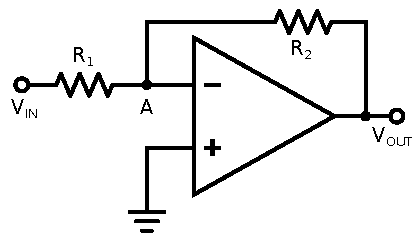
\includegraphics[width=.65\textwidth]{ccinv.pdf}
			\caption{Amplificatore invertente}
			\label{fig:ccinv}

		\end{minipage}%
		\hspace{10mm}%
		\begin{minipage}[c]{.4\textwidth}
			\centering

			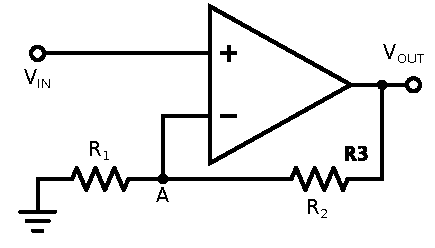
\includegraphics[width=.65\textwidth]{ccninv.pdf}
			\caption{Amplificatore non invertente}
			\label{fig:ccninv}
			
		\end{minipage}
\end{figure}

Il primo circuito da noi analizzato consiste in un amplificatore invertente accoppiato DC.
Come vediamo dallo schema riportato in Fig. \ref{fig:ccinv}, l'amplificatore operazionale è collegato con un circuito di \textbf{feedback negativo}.
Tale circuito, che collega l'uscita del circuito al contatto invertente dell'op-amp, ha lo scopo di contrastare il guadagno dell'integrato ($G_{op-amp} \approx 10^6$).
In questo modo si può avere un controllo sul segnale in uscita dall'amplificatore.
Senza tale circuito l'uscita del circuito avrebbe tensione $\pm V_{CCE}$ (cioè il massimo fornuto dall'alimentazione).

\begin{figure}[h!]
	\centering
			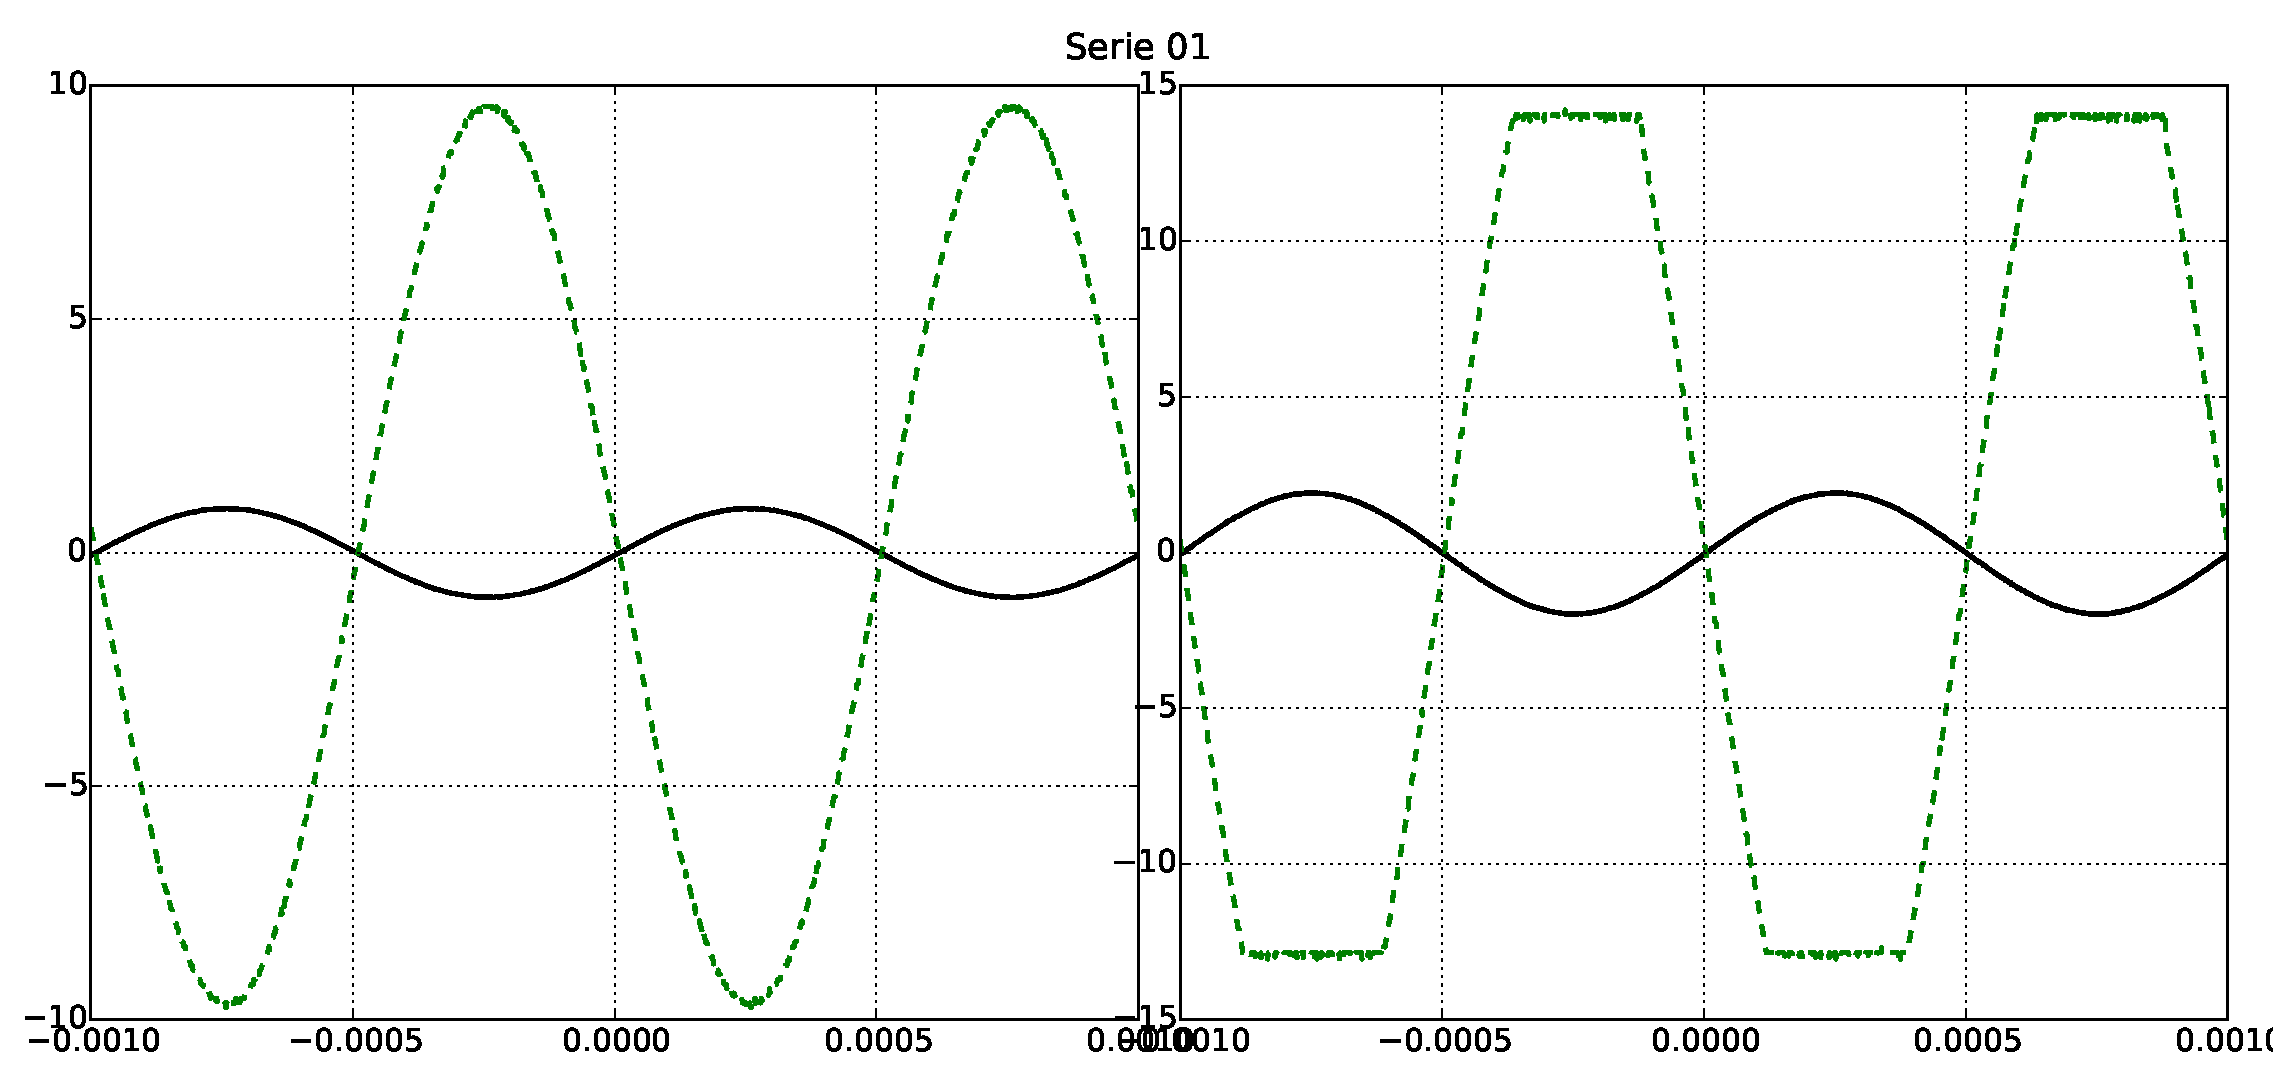
\includegraphics[width=\textwidth]{serie_01_ampl.pdf}
			\caption{In nero segnale in input e in verde segnale in output dell' amplificatore invertente. Nel grafico a destra possiamo apprezzare l'effetto di clipping. / Come vediamo il segnale in uscita non è più sfasato di $\pi$ ma risulta in fase con quello in input.}
			\label{fig:der}
\end{figure}

Se consideriamo il nostro amplificatore operazionale ideale, abbiamo che $\Delta V_{12}=0$ (I$^a$ condizione di idealità).
Il punto $A$ sarà un ground virtuale ($V_A = 0$).
Possiamo dunque imporre $I_1=\frac{V_{in}-V_A}{R_1}=\frac{V_{in}}{R_1}$.
Inoltre $I_2=\frac{V_A-V_{out}}{R_2}=\frac{-V_{out}}{R_2}$.
Sfruttando la II$^a$ condizione di idealità, $\Delta I_{12}=0$, otteniamo $V_{out}=-\frac{R_2}{R_1} V_{in}$.

Il guadagno del nostro circuito amplificatore sarà dunque:

\begin{equation}
G=-\frac{R_2}{R_1}
\end{equation}

Esso è negativo in quanto sfasato rispetto al segnale in ingresso di $\pi$.
La richiesta fatta era di ottenere un guadagno di circa -10.
Abbiamo dunque scelto di usare $R_1=(1001.6\pm0.3)\Omega$ e $R_2=(9987.1\pm0.3)\Omega$.
Il guadagno sperimentale ottenuto è stato di $-9.91 \pm 0.02$.

\begin{wrapfigure}[25]{r}[0pt]{.48\textwidth}
			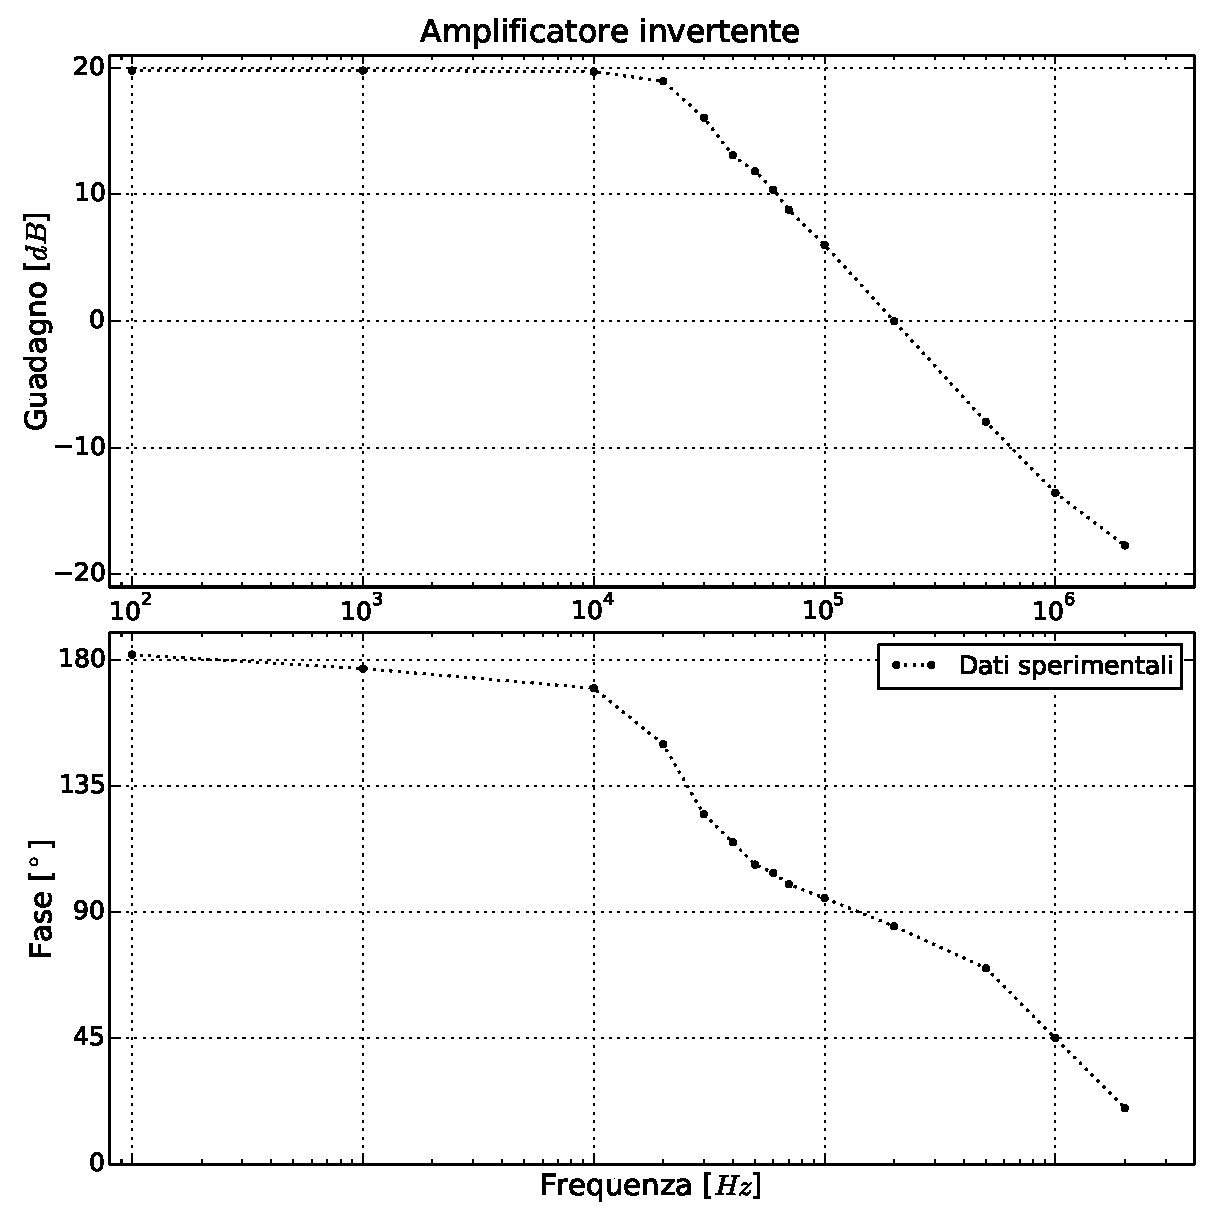
\includegraphics[width=.48\textwidth]{b_inv.pdf}
			\caption{Diagramma di Bode per l'amplificatore invertente}
			\label{fig:invbode}
\end{wrapfigure}

Il circuito è stato alimentato con un segnale in input sinusoidale alla frequenza di 1kHz.
Per valori picco-picco maggiori di $3V$ abbiamo notato l'ormai conosciuto effetto di clipping del segnale, in quanto la tensione in output raggiungeva il valore massimo fornito dalla polarizzazione DC dell'op-amp. 

Ne abbiamo inoltre analizzato l'andamento al variare della frequenza.
Come già accaduto per l'amplificatore alle differenze, abbiamo notato che a frequenze elevate il guadagno diminuiva considerevolmente, con anche uno sfasamento rilevante dei segnali.

In Fig. \ref{fig:invbode} è riportato un grafico del guadagno in funzione della frequenza. 

Crediamo che il motivo di tale comportamento %smorzamento
del segnale sia la presenza dei transistor e delle capacità nell'amplificatore operazionale.

Successivamente abbiamo montato il circuito dell'amplificatore non invertente, come mostrato in Fig. \ref{fig:ccninv}. Con gli stessi ragionamenti utilizzati per il precedente circuito, possiamo calcolare il guadagno di tale circuito: $V_A=V_{in}=V_{out}\frac{R_1}{R_2+R_1} \Rightarrow V_{out}=(1+\frac{R_2}{R_1})$. Il guadagno, positivo in questo caso, risulta essere: 

\begin{equation}
G=1+\frac{R_2}{R_1}
\end{equation}

Anche per questo circuito abbiamo analizzato la risposta in frequenza.
Il risultato ottenuto è molto simile a quello già mostrato per il circuito precedentemente analizzato e dunque abbiamo deciso di non riportarne il grafico. Il guadagno sperimentale ottenuto è stato di $10.97 \pm 0.2$.
